% ===================== PARTE 7: LATENCIA (diapositivas 70-79, más un anexo con p = 24) =====================
\parte{Latencia}{Latencia: la figura 6}
  {Cuánto tarda cada operación, con y sin competencia. Qué se sostiene, un error de compilación que casi se cuela y por qué las medianas con contención bailan tanto.}{s70}

\begin{frame}{Cómo se mide la latencia}
  \fuente{de Wolff et al., sección 6.2; EXPLICACION.md, Partes 4 y 6.2}
  \begin{columns}[T]
    \column{0.52\textwidth}
    \sub{El experimento}
    \begin{itemize}\small
      \item Corren $p$ hilos a la vez. El primero se cronometra; los demás hacen \texttt{store} sin parar, para crear contención.
      \item Tres operaciones: \texttt{load} (leer), \texttt{store} (escribir sin liberar) y \texttt{store \& reclaim} (escribir y liberar el objeto viejo).
      \item $p = 1$ (sin contención), 24 (todos los núcleos) y 56 (más hilos que núcleos).
      \item Binarios oficiales: 5 rondas con Docker y 15 sin Docker.
    \end{itemize}
    \column{0.44\textwidth}
    \sub{Cómo leer una caja}
    \centering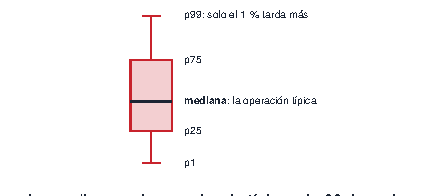
\includegraphics[width=0.95\linewidth]{figuras/s71}
    \par\raggedright\small
    La mediana es la experiencia típica; el p99, lo malo que puede ponerse.
  \end{columns}
  \nota{s71}
\end{frame}

\begin{frame}{Latencia con los binarios oficiales, con Docker}
  \fuente{docker/latencia.csv; mediana de 5 rondas de cada percentil}
  \centering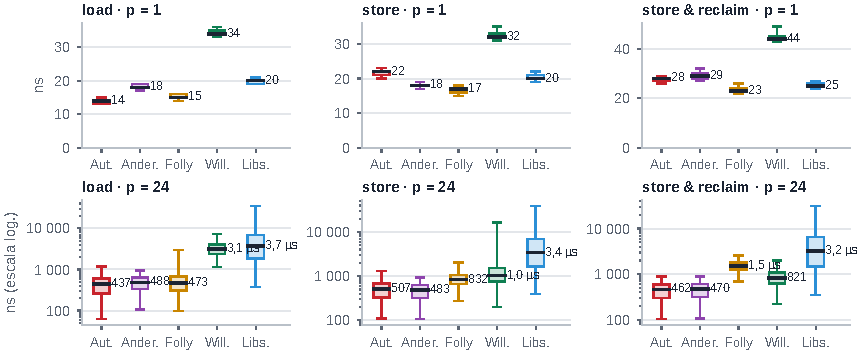
\includegraphics[width=\linewidth]{figuras/s72}
  \nota{s72}
\end{frame}

\begin{frame}{Medianas: réplica frente al paper}
  \fuente{docker/latencia.csv; valores del paper leídos de las etiquetas de su figura 6}
  \centering\footnotesize\renewcommand{\arraystretch}{1.08}
  \newcommand{\pp}{\quad\color{gris}paper}
  \begin{tabular}{@{}l*{5}{r}@{}}
    \toprule
    \textbf{Mediana, ns} & \textbf{Autores} & \textbf{Anderson} & \textbf{Folly} & \textbf{Williams} & \textbf{Libstdc++}\\
    \midrule
    \texttt{load}, $p = 1$ & \textbf{14} & 18 & 15 & 34 & 20\\
    \pp & \color{gris}23 & \color{gris}28 & \color{gris}24 & \color{gris}--- & \color{gris}29\\
    \texttt{load}, $p = 56$ & \textbf{1\,502} & 1\,540 & 2\,977 & 23\,738 & 61\,687\\
    \pp & \color{gris}1\,140 & \color{gris}2\,580 & \color{gris}11\,600 & \color{gris}--- & \color{gris}99\,700\\
    \texttt{store}, $p = 1$ & 22 & 18 & \textbf{17} & 32 & 20\\
    \pp & \color{gris}33 & \color{gris}28 & \color{gris}37 & \color{gris}--- & \color{gris}36\\
    \texttt{store}, $p = 56$ & 1\,516 & \textbf{1\,498} & 4\,813 & 4\,105 & 52\,832\\
    \pp & \color{gris}1\,470 & \color{gris}2\,840 & \color{gris}2\,620 & \color{gris}--- & \color{gris}111\,000\\
    \texttt{store \& reclaim}, $p = 1$ & 28 & 29 & \textbf{23} & 44 & 25\\
    \pp & \color{gris}44 & \color{gris}44 & \color{gris}49 & \color{gris}--- & \color{gris}41\\
    \texttt{store \& reclaim}, $p = 56$ & \textbf{813} & 1\,499 & 6\,525 & 4\,439 & 47\,198\\
    \pp & \color{gris}1\,570 & \color{gris}1\,250 & \color{gris}5\,060 & \color{gris}--- & \color{gris}59\,300\\
    \bottomrule
  \end{tabular}
  \par\smallskip\raggedright\scriptsize
  En negrita, la mejor de cada fila de la réplica. El paper no publica la latencia de Williams. Con $p = 24$, ver el \hyperlink{anexop24}{anexo}.
  \nota{s73}
\end{frame}

\begin{frame}{Cada rival respecto a Autores: paper frente a réplica}
  \fuente{docker y nativo\_oficial/latencia.csv; figura 6 del paper; $p = 56$ en los dos}
  \centering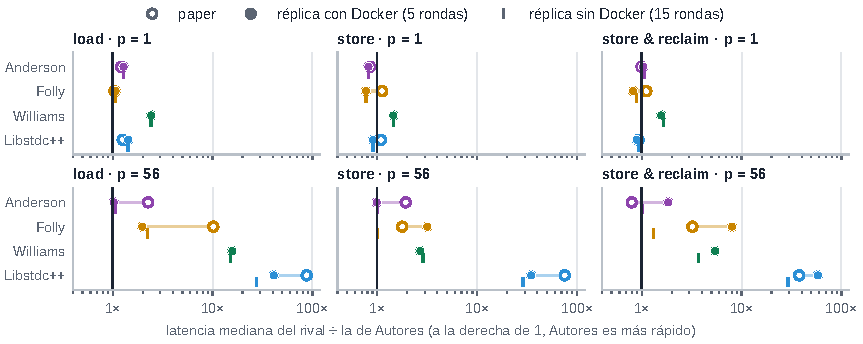
\includegraphics[width=\linewidth]{figuras/s74}
  \nota{s74}
\end{frame}

\begin{frame}{Lo que se sostiene en latencia, y lo que no}
  \fuente{docker y nativo\_oficial/latencia.csv; EXPLICACION.md, Partes 6.2 y 7}
  \footnotesize\renewcommand{\arraystretch}{1.2}
  \begin{tabularx}{\linewidth}{@{}p{0.33\linewidth}Xp{0.15\linewidth}@{}}
    \toprule
    \textbf{Lo que dice el paper} & \textbf{Lo que sale aquí, con y sin Docker} & \textbf{Veredicto}\\
    \midrule
    7. El \texttt{load} de Autores es siempre el de menor latencia & El más bajo en los tres casos. Con contención, por un 8-12\,\% frente a Folly y Anderson; con $p = 56$, empate con Anderson & \sirep\newline{\scriptsize\color{gris}por poco}\\
    8. El \texttt{store} de Autores es el segundo con $p = 1$ & Es el cuarto de cinco, por 5\,ns & \norep\\
    9. El \texttt{store} de Autores es el mejor con contención & Empate con Anderson: 507 frente a 483\,ns con $p = 24$; sin Docker, 461 frente a 470 & \enparte\\
    10. \texttt{store \& reclaim} es más lento que \texttt{store} con $p = 1$ & Los cinco & \sirep\\
    11. Con contención, algunos van más rápido en \texttt{store \& reclaim} & Con Docker, Autores baja de 1\,516 a 813\,ns con $p = 56$. Sin Docker y 15 rondas, solo un 1-4\,\%: dentro del ruido & \noconf\\
    12. La latencia de Williams es casi siempre mayor & Sin contención, la mayor en las 3 operaciones. Con contención supera a Libstdc++ en 6 de 6 y a Folly en 3 de 6 (sin Docker, 5 y 2) & \enparte\\
    \bottomrule
  \end{tabularx}
  \nota{s75}
\end{frame}

\begin{frame}{Una trampa que casi se cuela: el candado escondido de Williams}
  \fuente{docker/latencia\_williams\_con\_candado.csv y latencia.csv; EXPLICACION.md, Parte 6.2}
  \begin{columns}[T]
    \column{0.47\textwidth}
    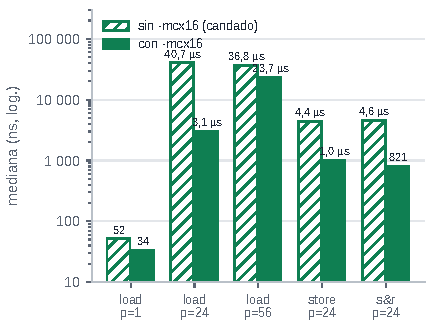
\includegraphics[width=\linewidth]{figuras/s76}
    \column{0.49\textwidth}
    \sub{Qué pasó}\footnotesize
    La primera medida decía que el \texttt{load} de Williams con $p = 24$ tardaba 40,7\,\textmu s, 93 veces más que Autores. Parecía confirmar al paper. \textbf{Era un error nuestro.}
    \par\medskip
    \porque{\texttt{-mcx16}}{Williams guarda 16 bytes y necesita la instrucción \texttt{cmpxchg16b}. El compilador solo la usa con \texttt{-mcx16}. El binario de latencia del artefacto se compila sin ella, y \texttt{boost::atomic} recurre en silencio a un candado interno.}
    \par\medskip
    \sub{Cómo se confirmó}\footnotesize
    Mirando el binario: llamadas a \texttt{lock\_pool} y ni un \texttt{cmpxchg16b}. Con \texttt{-mcx16}: 0 llamadas y 10 instrucciones.
  \end{columns}
  \nota{s76}
\end{frame}

\begin{frame}{Las colas: lo que la mediana no cuenta}
  \fuente{docker/latencia.csv; mediana de 5 rondas de cada percentil}
  \centering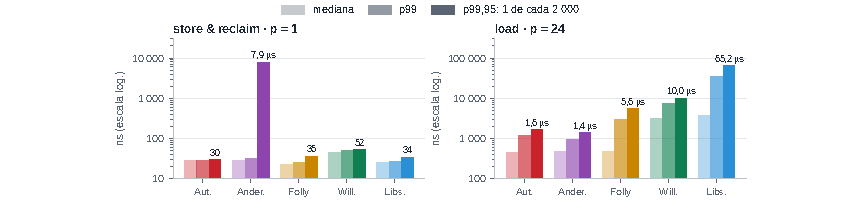
\includegraphics[width=0.9\linewidth]{figuras/s77}
  \par\medskip\raggedright
  \begin{columns}[T]
    \column{0.49\textwidth}
    \porque{la caja de pendientes de Anderson}{Anderson vacía su caja cada 2\,000 retiradas y recorre las mesas de todos. 1 de cada 2\,000 es el 0,05\,\%: justo lo que mira el p99,95, que salta de 32 a casi 8\,000\,ns. No se midió directamente.}
    \column{0.47\textwidth}
    \porque{lock-free no es wait-free}{Con 23 escritores, el \texttt{load} de Williams necesita ganar dos bucles de CAS. El sistema avanza, pero el lector se queda atrás: 1 lectura de cada 2\,000 tarda 10\,\textmu s; en Autores, 1,6\,\textmu s.}
  \end{columns}
  \nota{s77}
\end{frame}

\begin{frame}{¿Cuánto fiarse de una mediana con contención? Poco}
  \fuente{docker y nativo\_oficial/latencia.csv; ronda más lenta ÷ más rápida de cada punto}
  \centering\scriptsize
  \alg{cAutores}{Autores}\quad\alg{cAnderson}{Anderson}\quad\alg{cFolly}{Folly}\quad\alg{cWilliams}{Williams}\quad\alg{cLibs}{Libstdc++}\qquad
  \tikz\fill[gris] (0,0) circle (2pt);~Docker, 5 rondas\quad\tikz\draw[gris] (0,0) circle (2pt);~sin Docker, 15 rondas
  \par\smallskip
  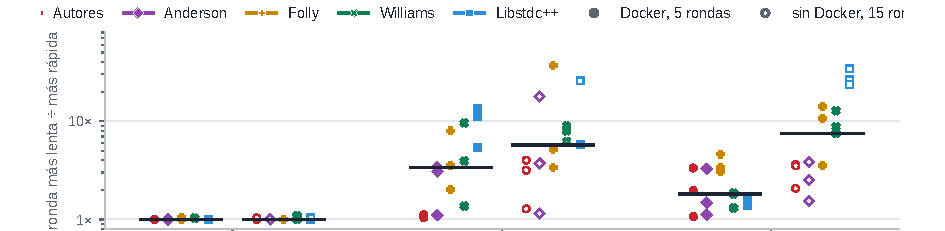
\includegraphics[width=\linewidth,trim=0 0 0 17,clip]{figuras/s78}
  \par\smallskip\footnotesize\renewcommand{\arraystretch}{1.12}
  \begin{tabular}{@{}lrrr@{}}
    \toprule
    \textbf{Ronda más lenta ÷ más rápida, mediana} & \textbf{Docker, 5 rondas} & \textbf{Sin Docker, 15 rondas} & \textbf{\texttt{bench.cpp}, 5 rondas}\\
    \midrule
    $p = 1$ & 1,00\por & 1,00\por & 1,11\por\\
    $p = 24$ & 3,40\por{} (peor, 13,6\por) & 5,75\por{} (peor, 36,9\por) & 1,84\por{} (peor, 10,4\por)\\
    \bottomrule
  \end{tabular}
  \nota{s78}
\end{frame}

\begin{frame}{Con $p = 24$, las rondas caen en dos grupos}
  \fuente{nativo\_oficial/latencia.csv, 15 rondas; EXPLICACION.md, Parte 6.2}
  \begin{columns}[T]
    \column{0.47\textwidth}
    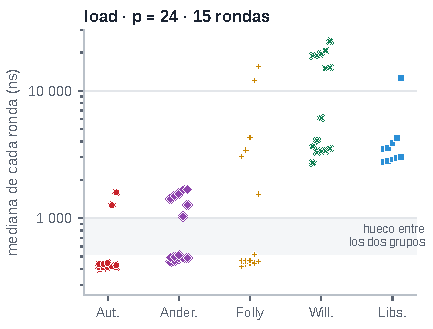
\includegraphics[width=\linewidth]{figuras/s79}
    \column{0.49\textwidth}
    \begin{itemize}\footnotesize
      \item Unas rondas quedan por debajo de 520\,ns y otras por encima de 1\,000\,ns, sin nada en medio.
      \item En el grupo rápido: Autores entre 399 y 445\,ns, Folly entre 420 y 517 y Anderson entre 451 y 511.
      \item Autores cae menos veces en el grupo lento: 2 de 15, frente a 6 de Folly y 7 de Anderson. Con 15 rondas no basta para llamarlo propiedad del algoritmo.
    \end{itemize}
    \medskip
    \caja{Con los hilos fijados (\texttt{todos24}) el grupo lento no apareció: 419-427\,ns en Autores. Indicio de que depende de dónde coloca Linux al hilo medido, en un núcleo P o E.}
  \end{columns}
  \nota{s79}
\end{frame}

\begin{frame}{Anexo de latencia: medianas y colas con $p = 24$}\label{anexop24}
  \fuente{resultados/david-ultra9-285/tablas.md, «Latencia: medianas en ns» y «Colas de latencia»; con Docker}
  \centering\footnotesize\renewcommand{\arraystretch}{1.15}
  \begin{tabular}{@{}l*{5}{r}@{}}
    \toprule
    \textbf{$p = 24$, ns: p50 / p99} & \textbf{Autores} & \textbf{Anderson} & \textbf{Folly} & \textbf{Williams} & \textbf{Libstdc++}\\
    \midrule
    \texttt{load} & \textbf{437} / 1\,175 & 488 / \textbf{952} & 473 / 3\,008 & 3\,104 / 7\,251 & 3\,716 / 34\,847\\
    \texttt{store} & 507 / 1\,321 & \textbf{483} / \textbf{926} & 832 / 2\,056 & 1\,021 / 16\,593 & 3\,411 / 38\,851\\
    \texttt{store \& reclaim} & \textbf{462} / \textbf{881} & 470 / 894 & 1\,521 / 2\,559 & 821 / 1\,977 & 3\,248 / 31\,386\\
    \bottomrule
  \end{tabular}
  \par\bigskip\raggedright
  \caja{Con todos los núcleos ocupados, Autores y Anderson quedan a menos de un 10\,\% en la mediana; en la cola, Anderson es algo mejor en \texttt{load} y \texttt{store}. Libstdc++ queda entre 7 y 9 veces por detrás en la mediana y unas 30 en el p99.}
  \note{Esta tabla completa la de las medianas con p igual a 24, que son todos los núcleos reales de la máquina.

Con contención, Autores y Anderson están muy cerca: en la mediana se separan menos de un diez por ciento, y en la cola Anderson es algo mejor al leer y al escribir. Libstdc++ queda muy atrás: entre siete y nueve veces en la mediana, y unas treinta veces en el p99.

Recuerden la regla de la parte 10: una diferencia pequeña con contención es un empate.
}
\end{frame}
